\chapter{System Model}
\label{cha:system}
\vspace{0.4 cm}

In this chapter, the model of the proposed system is presented.
In the first section, an in-depth presentation of the system architecture is provided.
The different components of the system with their functionalities and the interactions among them are described.
Lastly, the three modules focused on the three use cases of interest are treated more in detail in dedicated sections.
After this chapter, it will be clear what the main parts of this system are and how they cooperate to achieve the various use cases of interest.


\section{System architecture}
\label{sec:architecture}
\vspace{0.2 cm}

Describe the system architecture and the different diagrams ...

\begin{figure}[H]
\centering 
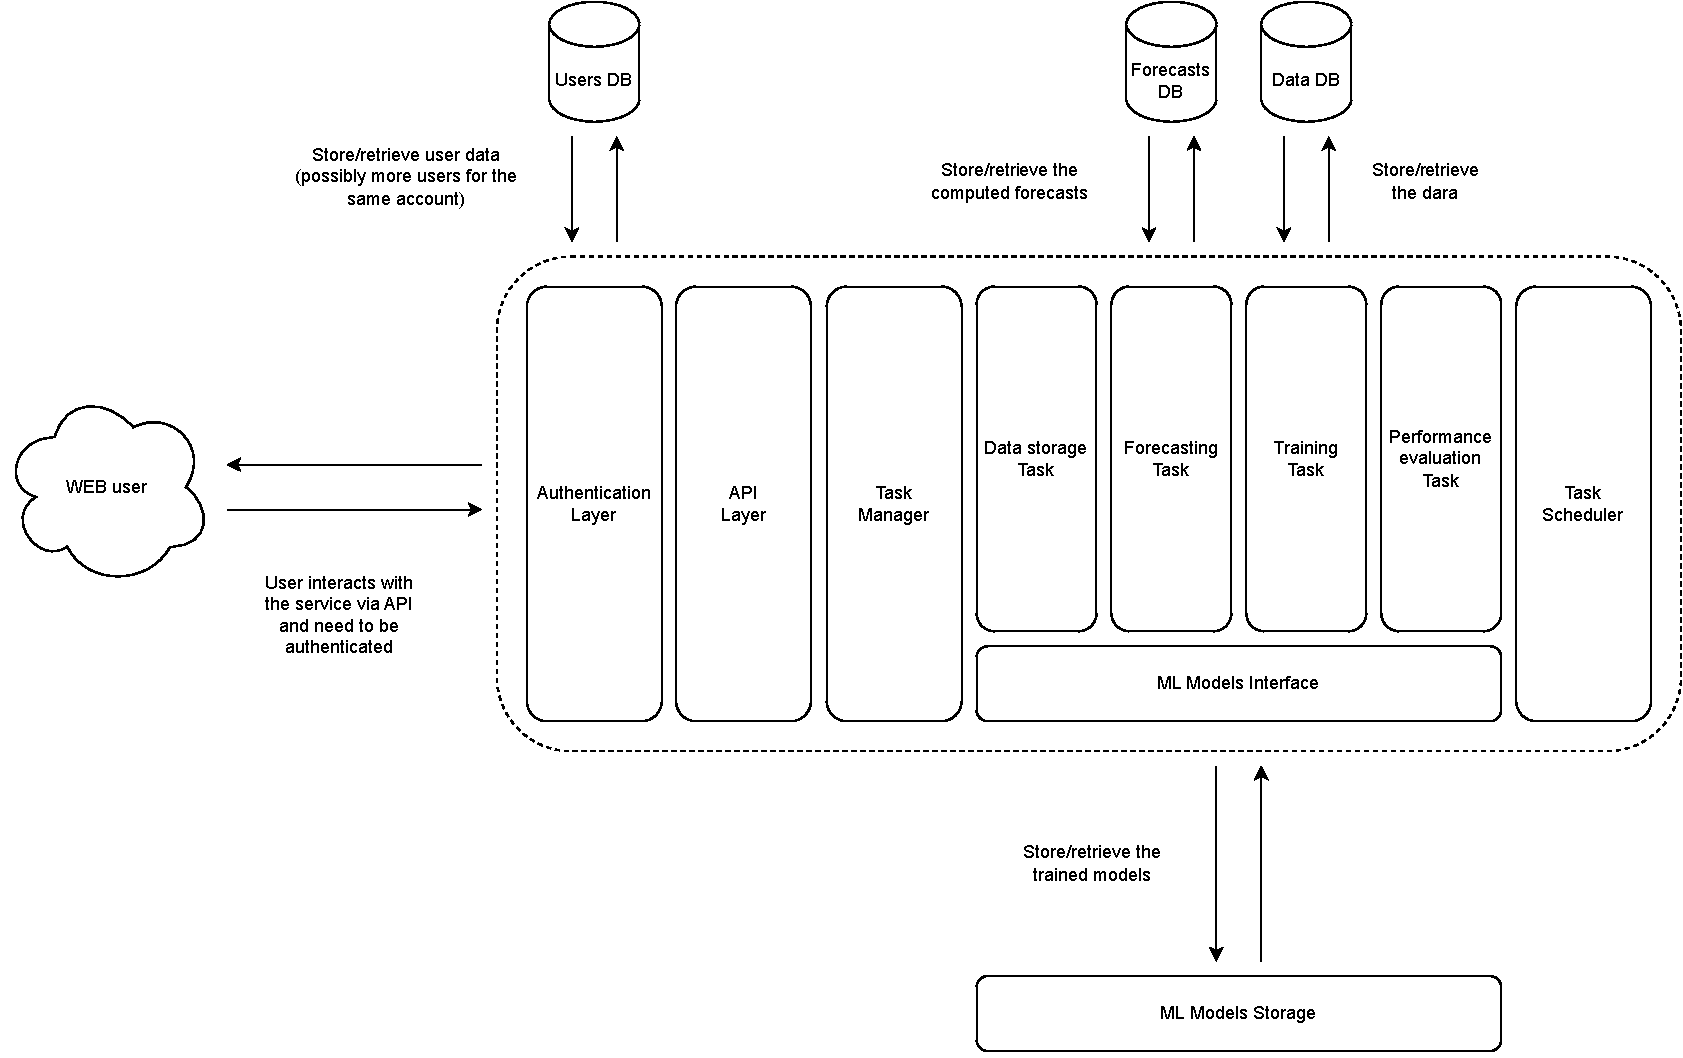
\includegraphics[width=0.9\textwidth]{images/architecture_components} 
\caption{The architecture of the proposed system.}
\label{fig:components}
\end{figure}

\begin{figure}[H]
\centering 
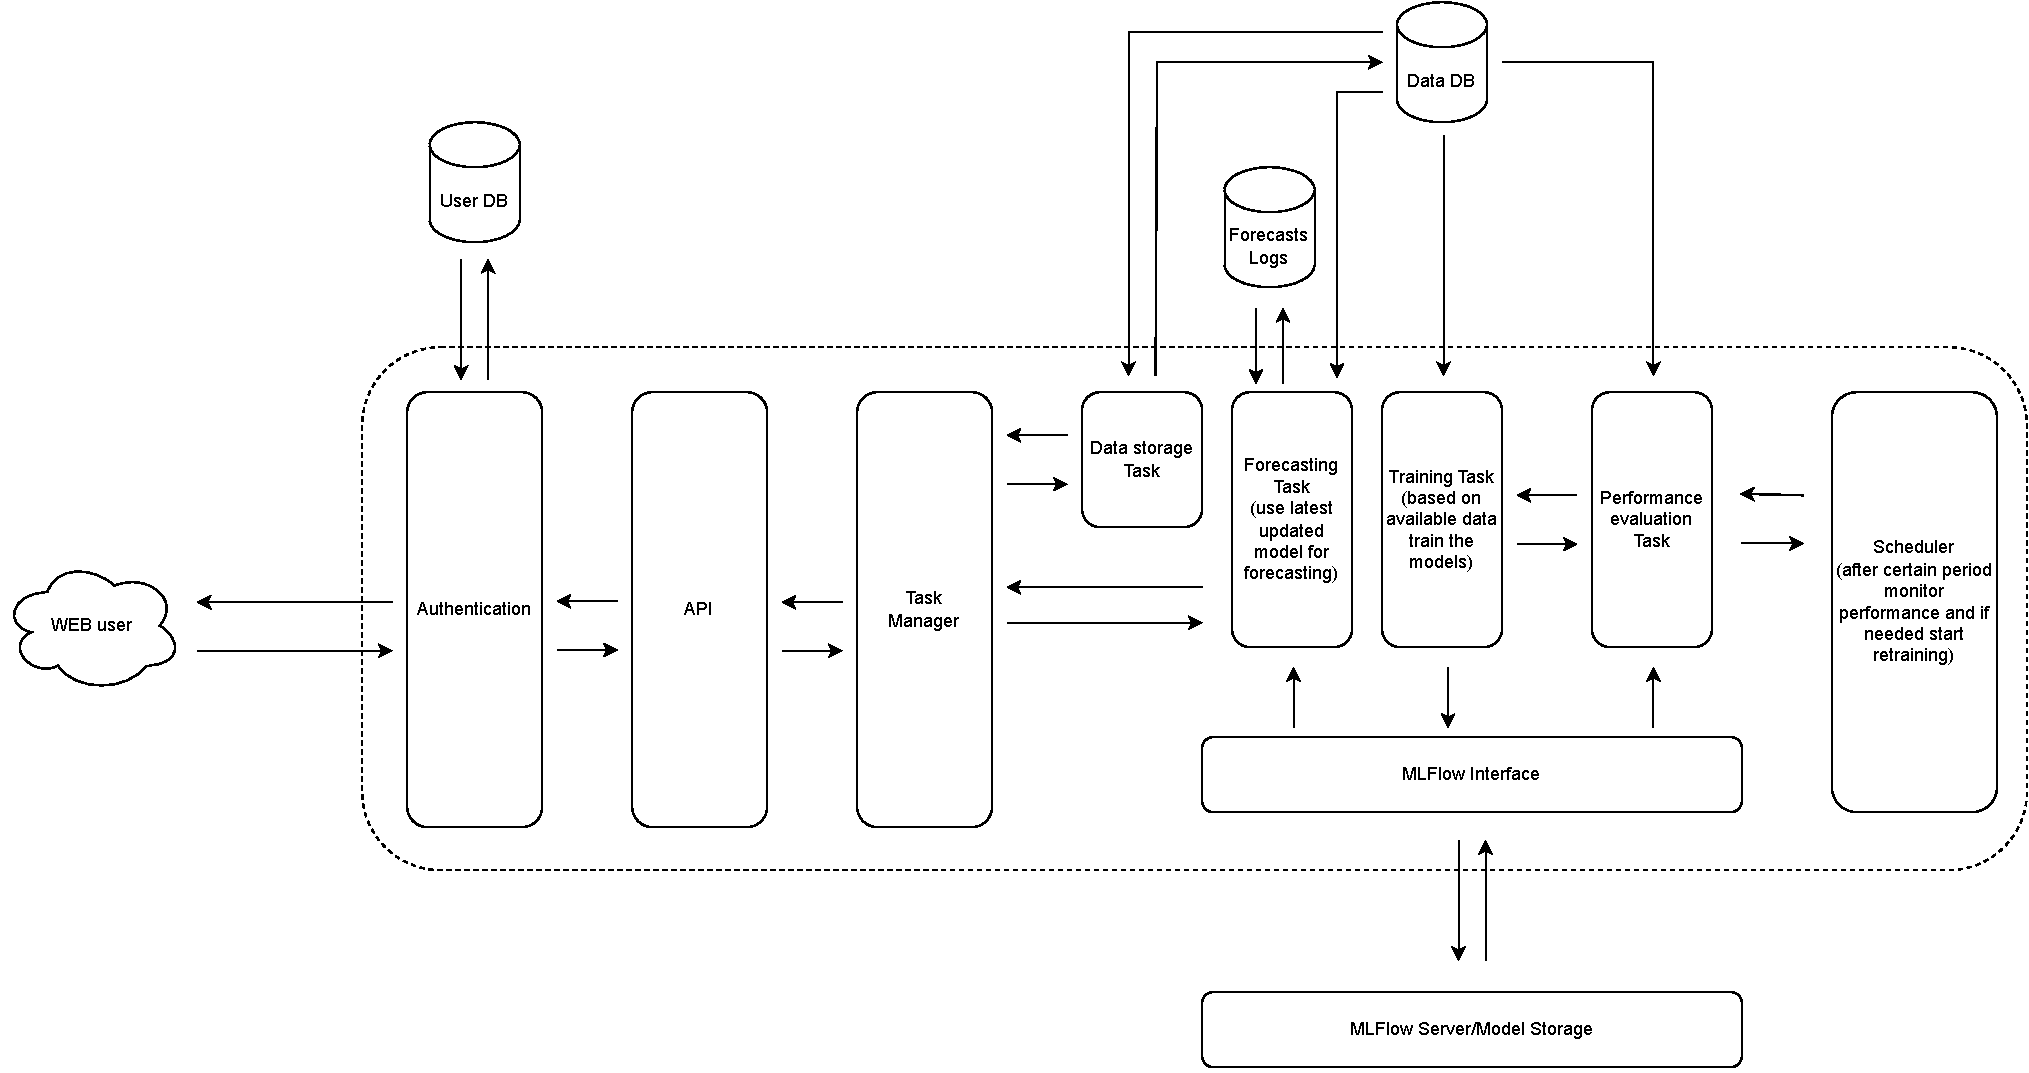
\includegraphics[width=1\textwidth]{images/architecture_interactions} 
\caption{The interactions of the components of the proposed system.}
\label{fig:interactions}
\end{figure}

\begin{figure}[H]
\centering 
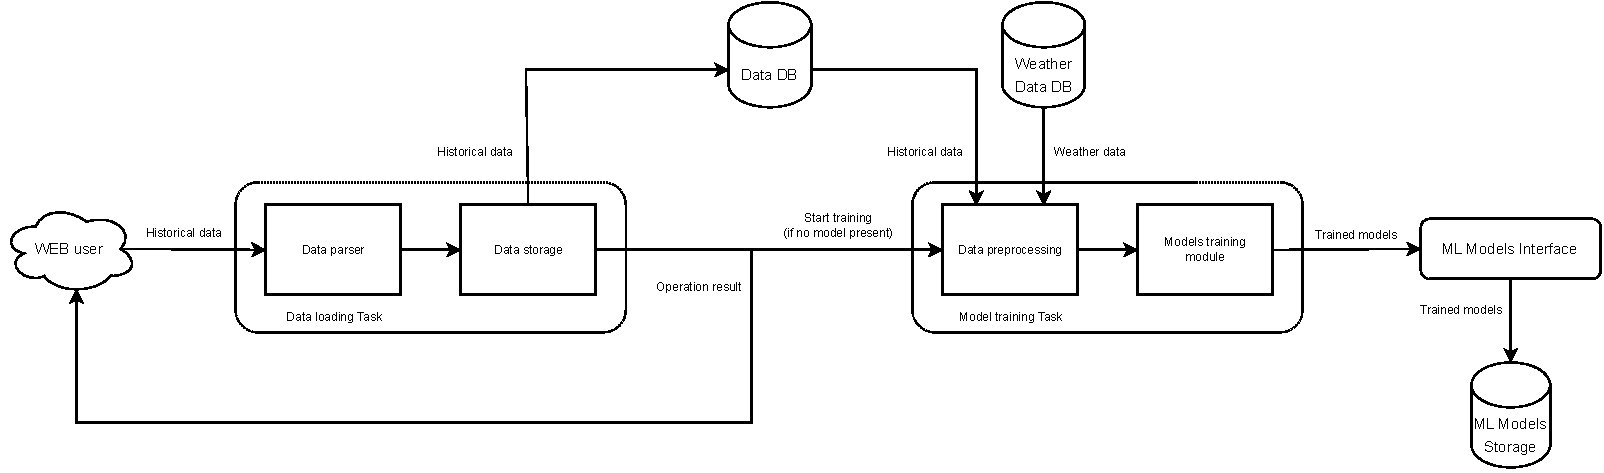
\includegraphics[width=1\textwidth]{images/architecture_data_loading_flow} 
\caption{Diagram representing the data loading flow.}
\label{fig:loadingflow}
\end{figure}

\begin{figure}[H]
\centering 
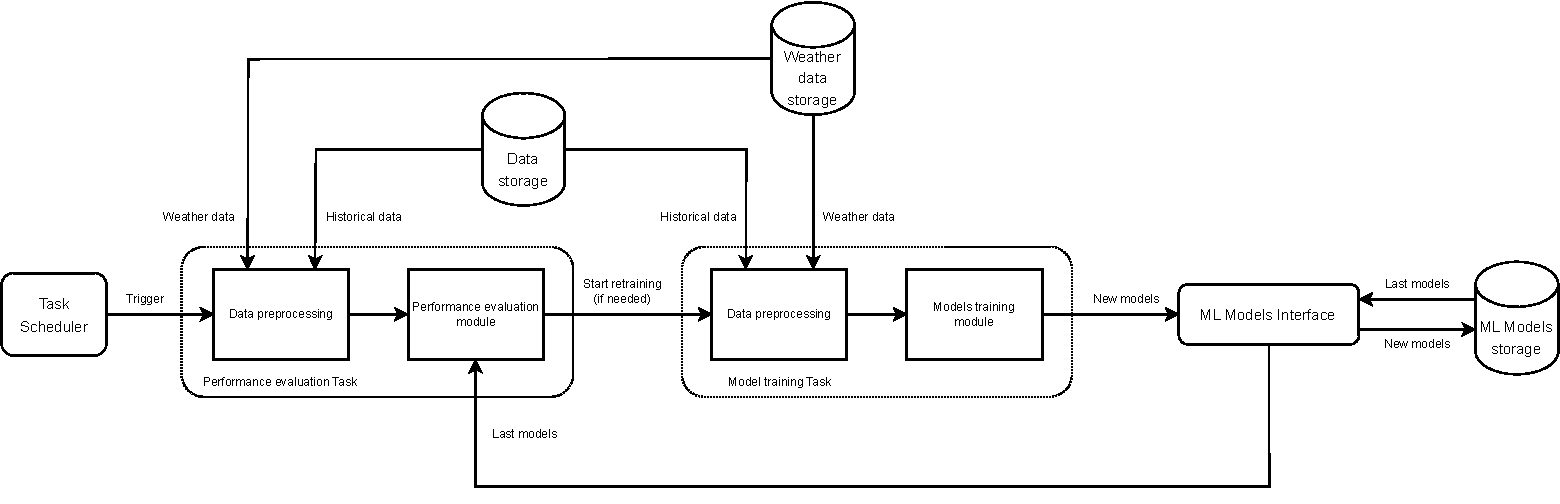
\includegraphics[width=0.85\textwidth]{images/architecture_scheduler_flow} 
\caption{Diagram representing the scheduler flow.}
\label{fig:schedulerflow}
\end{figure}

\begin{figure}[H]
\centering 
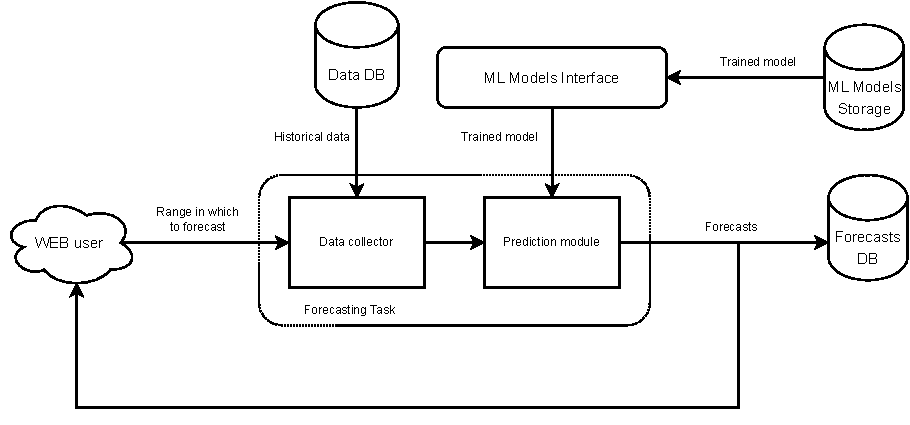
\includegraphics[width=0.65\textwidth]{images/architecture_forecast_flow} 
\caption{Diagram representing the forecast flow.}
\label{fig:forecastflow}
\end{figure}

\begin{figure}[H]
\centering 
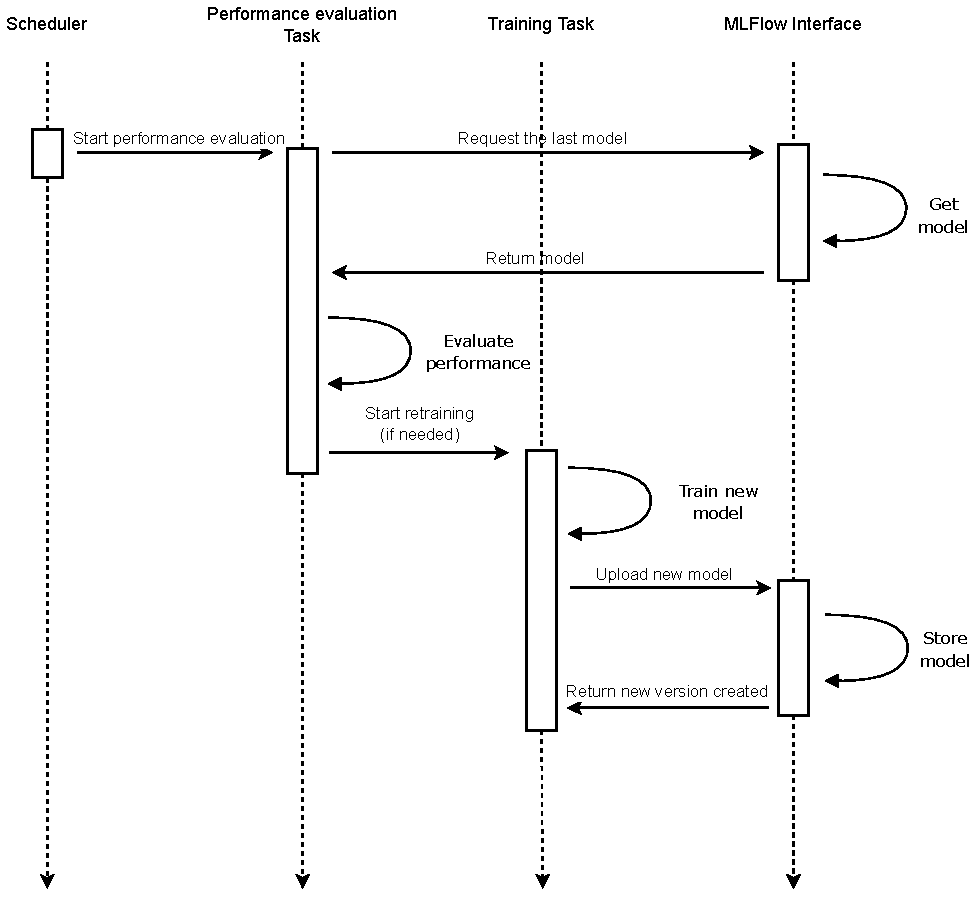
\includegraphics[width=0.5\textwidth]{images/architecture_scheduler_sequence} 
\caption{Diagram representing the scheduler sequence diagram.}
\label{fig:schedulersequence}
\end{figure}

\begin{figure}[H]
\centering 
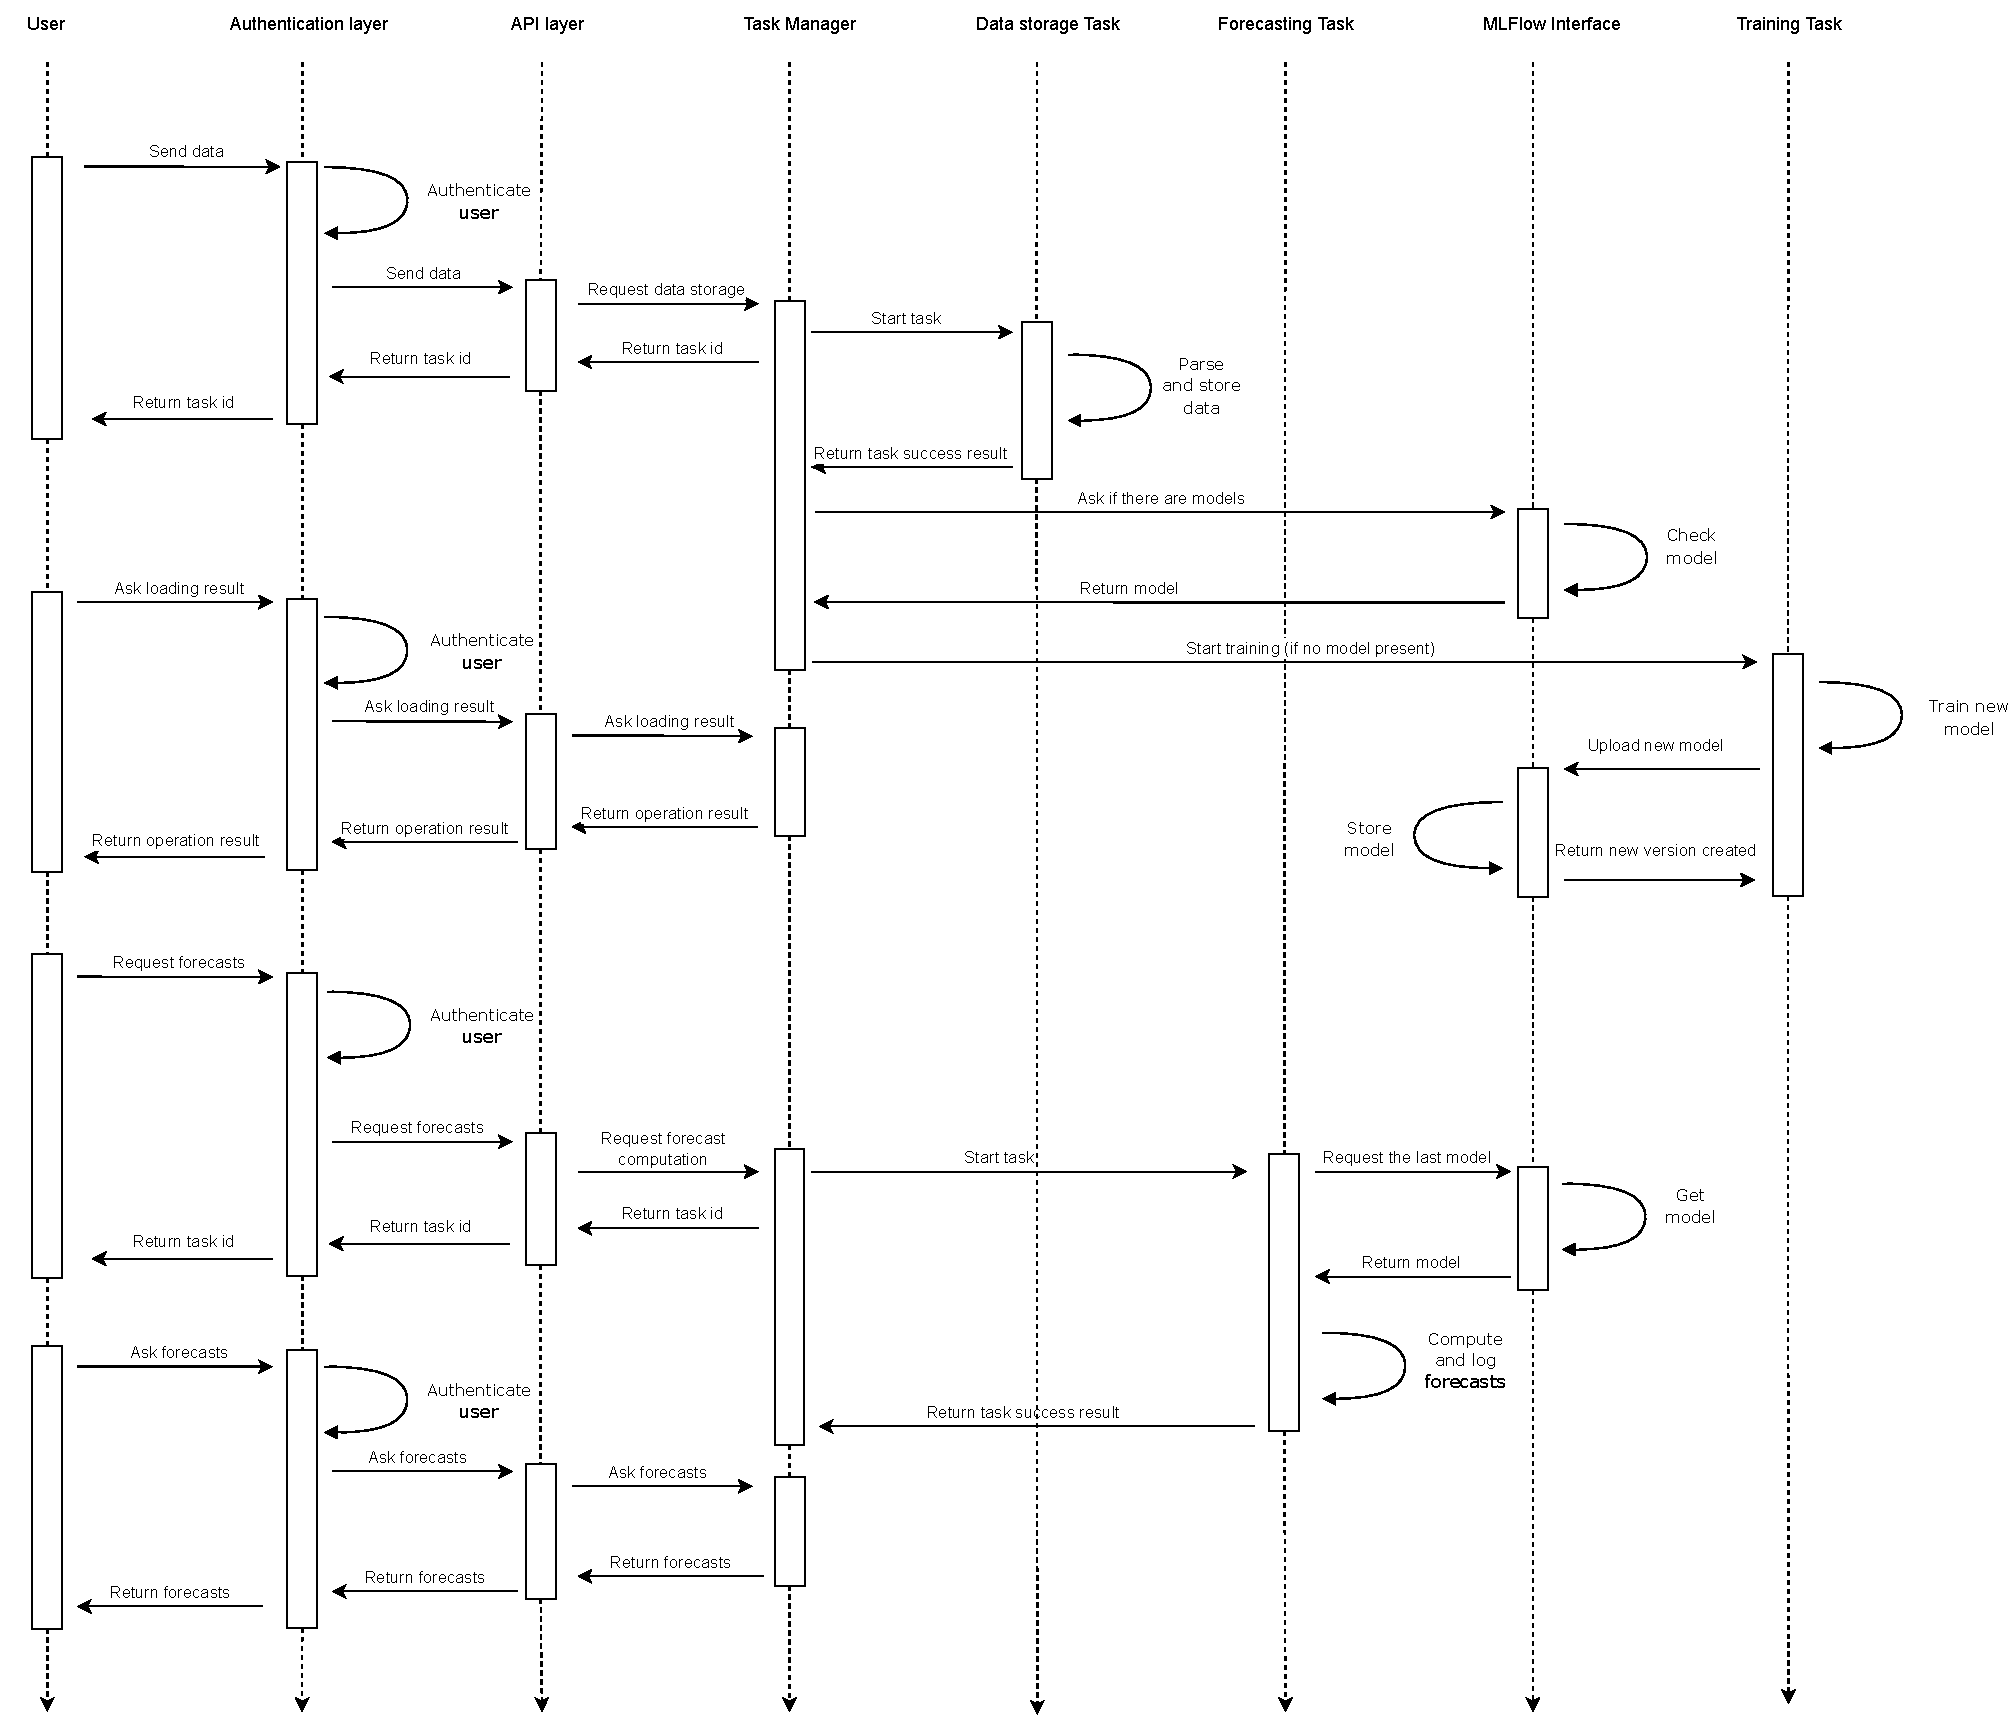
\includegraphics[width=1\textwidth]{images/architecture_user_sequence} 
\caption{Diagram representing the user sequence diagram.}
\label{fig:usersequence}
\end{figure}

\begin{figure}[H]
\centering 
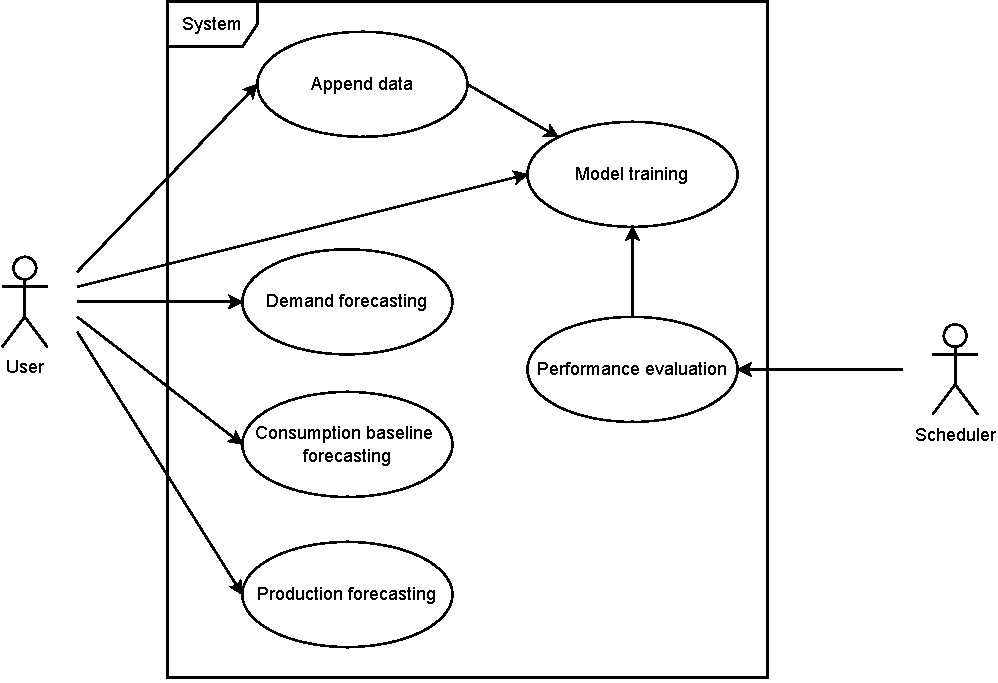
\includegraphics[width=0.65\textwidth]{images/architecture_use_case} 
\caption{The use case diagram for the system.}
\label{fig:usecase}
\end{figure}


\section{System common components}
\label{sec:components}
\vspace{0.2 cm}

Describe the system's common components between the various tasks ...

\begin{figure}[H]
\centering 
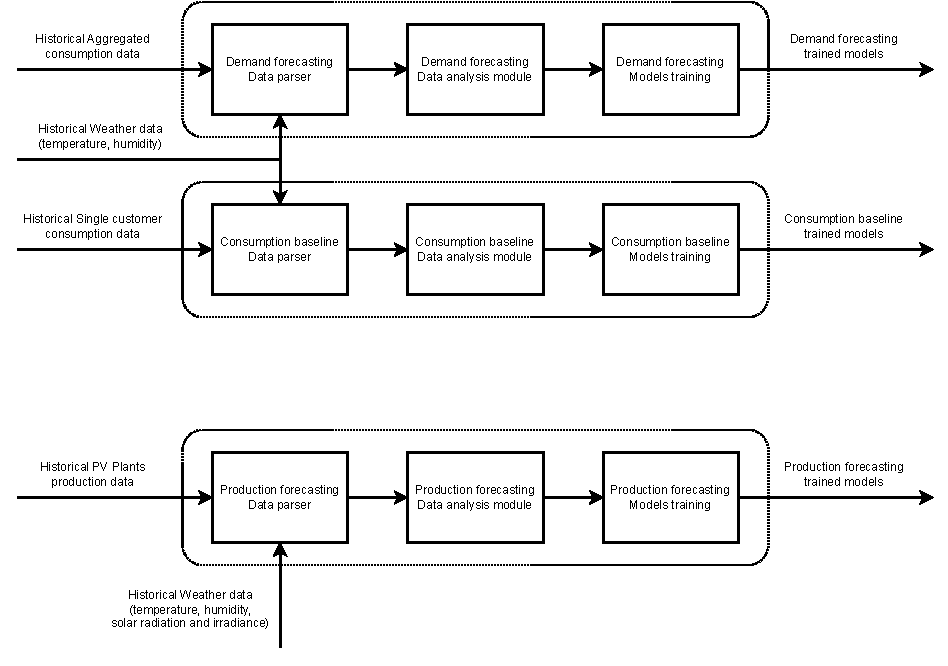
\includegraphics[width=1\textwidth]{images/system_model_training} 
\caption{The system model training schematic representation.}
\label{fig:modeltraining}
\end{figure}

\begin{figure}[H]
\centering 
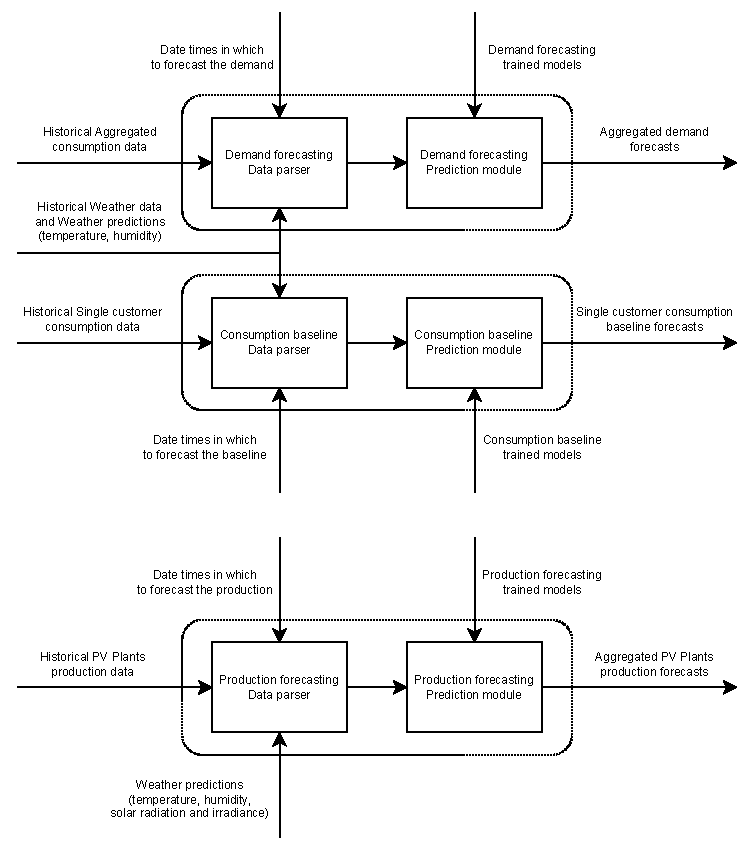
\includegraphics[width=0.8\textwidth]{images/system_model_forecasting} 
\caption{The system model forecasting schematic representation.}
\label{fig:modelforecasting}
\end{figure}


\section{Electricity demand forecasting module}
\label{sec:demandmodel}
\vspace{0.2 cm}

Describe the electricity demand forecasting module ...


\section{Consumption baseline forecasting module}
\label{sec:baselinemodel}
\vspace{0.2 cm}

Describe the consumption baseline forecasting module ...


\section{Electricity production forecasting module}
\label{sec:productionmodel}
\vspace{0.2 cm}

Describe the electricity production forecasting module ...
